\documentclass[10pt,a4paper]{article}
\usepackage{graphicx}
\usepackage{hyperref}
\usepackage[utf8x]{inputenc}
\usepackage{polski}

\begin{document}

\begin{titlepage}
\begin{center}


\includegraphics[scale=0.25]{../../common/sakuralogo.png}
\vfill

\huge
4MB PCMCIA SRAM

Instrukcja Obsługi

\vspace*{1cm}

\normalsize
Tanie rozszerzenie Fast RAM dla Amigi 600/1200.

\vspace*{5cm}

\today

\end{center}
\end{titlepage}

\section*{Opis}

Dziękujemy za zakup rozszerzenia Sakura 4MB PCMCIA SRAM! Ten produkt ma następujące właściwości:

\begin{itemize}
	\item Rozszerza Amigę 600 lub 1200 o 4MB pamięci Fast RAM.
	\item Przyśpiesza nierozszerzoną Amigę 1200 do przynajmniej 1.67 MIPS (według SysInfo).
	\item Jest zbudowany z użyciem nowoczesnych, szybkich układów SRAM o czasie dostępu 55ns.
	\item Bardzo prosta instalacja - zwyczajnie włóż kartę w slot PCMCIA po lewej stronie Amigi.
	\item Kompatybilny z wszystkimi akceleratorami oraz rozszerzeniami pamięci przyjaznymi dla slotu PCMCIA\footnote{Zrobiliśmy wiele aby zapewnić działanie karty w największej możliwej ilości konfiguracji, ale niektóre akceleratory oraz rozszerzenia Fast RAM są z założenia niekompatybilne ze slotem PCMCIA jeśli zainstalowane jest więcej niż 4MB pamięci. Karta PCMCIA SRAM powinna działać z nimi tak czy inaczej, jeśli na owym rozszerzeniu zainstalowane jest 4MB pamięci lub mniej. Oczywiście, jeśli nie masz żadnego akceleratora ani rozszerzenia pamięci, to nie musisz się tym przejmować.}.
	\item Otwarty projekt\footnote{Odwiedź repozytorium kodu źródłowego: \url{https://github.com/rkujawa/ppa-pcmcia-sram} .} na licencji CC-BY-SA (płytka) oraz MIT (wsad CPLD).
	\item Stworzony przez Amigowców dla Amigowców! 
\end{itemize}

%To reduce the price, card is delivered without any kind of case. The case might be available in the future from 3rd party vendor.

\section*{Instalacja}

Procedura instalacji jest bardzo prosta. Aby zainstalować rozszerzenie wykonaj następujące kroki:

\begin{itemize}
	\item Wyłącz swoją Amigę.
	\item Wsuń kartę do slotu PCMCIA, zlokalizowanego po lewej stronie Twojego komputera. 
	%The card's components should be facing upwards.
	\item Upewnij się że przełącznik {\tt RAM/disk} jest ustawiony w pozycji {\tt RAM}.
	\item Włącz swoją Amigę i rozkoszuj się dodatkowymi 4MB pamięci.
\end{itemize}

Twoja Amiga powinna uruchomić się jak zazwyczaj, jednak nieco szybciej. Po instalacji możesz potwierdzić, że rozszerzenie działa prawidłowo, poprzez sprawdzenie ilości dostępnej pamięci na górnej belce Workbench'a, albo używając komendy {\tt avail} lub {\tt ShowConfig}. Popularne narzędzie SysInfo zaraportuje dodatkowe 4MB pamięci pod nazwą {\tt card.resource}.

\section*{Szczegóły techniczne}

\begin{center}
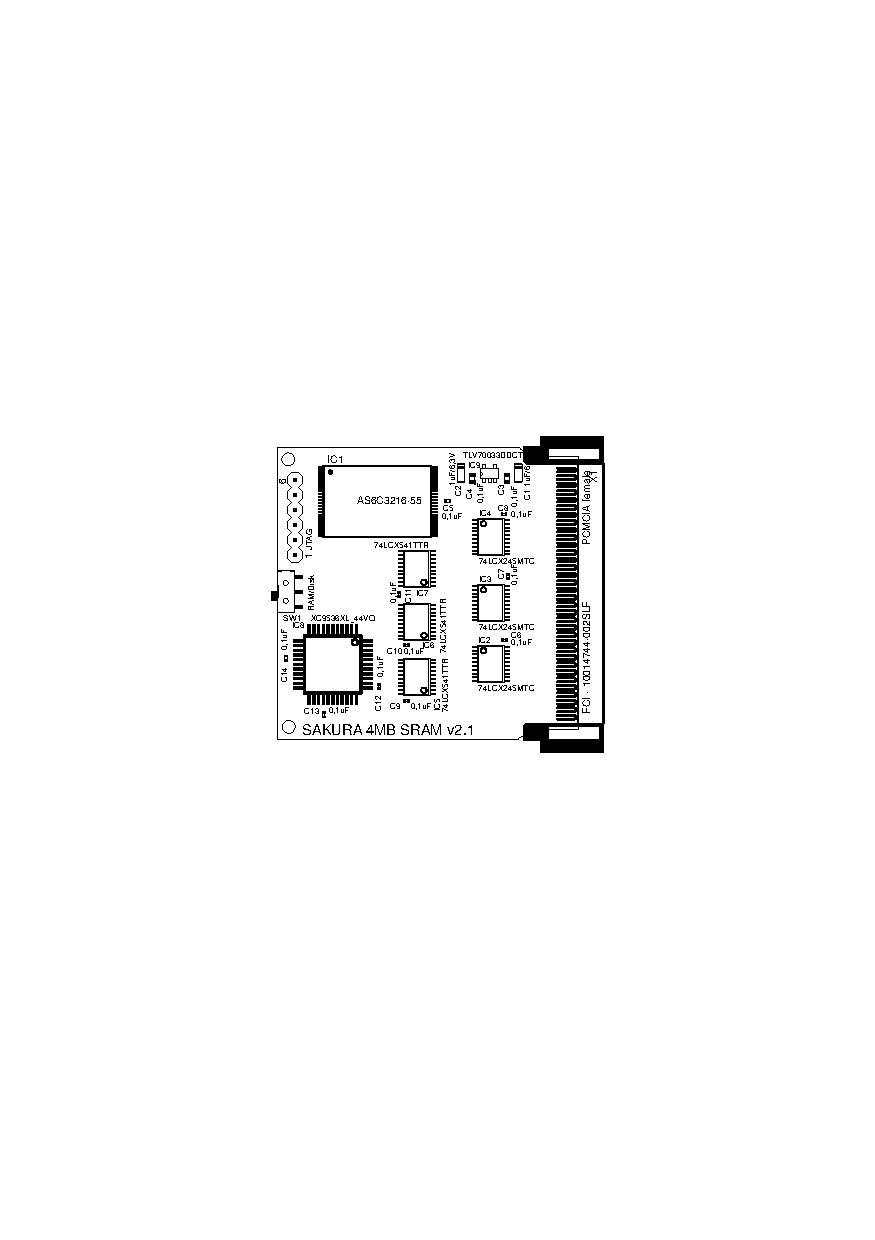
\includegraphics{board21layout.pdf}
\end{center}

Karty Sakura w rewizji 2.x są zbudowane w oparciu o układ Alliance Memory AS6C3216, który jest 32-megabitowym układem SRAM z 16-bitową szyną danych, o czasie dostępu 55ns. Pamięć jest dostępna w górnych 4MB przestrzeni Zorro 2 ({\tt 0x600000-0x9FFFFF}).

Sygnały kontrolne dla układu SRAM są generowane przez CPLD Xilinx XC9536XL, bazując na sygnałach dostępu do slotu PCMCIA.

To rozszerzenie jest konfigurowane w pełni automatycznie. Pamięć jest dodawana do systemowej puli pamięci przez Kickstart. Proces automatycznej konfiguracji jest wykonywany zgodnie z danymi przedstawianymi przez kartę w strukturze CIS (ang. Card Information Structure), które jest analizowana przez {\tt card.resource}. Naturalnie, ten proces ma miejsce jedynie podczas startu systemu, więc włożenie karty do Amigi podczas jej pracy nie powoduje automatycznego dodania pamięci. Jeśli jest to konieczne, istnieje możliwość ręcznego dodania pamięci za pomocą komendy {\tt AddMem} (dostępnej na aminecie), jednakże to nie jest wymagane podczas normalnej pracy. 

CIS rozszerzenia Sakura zawiera optymalne ustawienia, ktore pozwalają na uzyskanie optymalnej wydajności slotu PCMCIA:
\begin{itemize}
	\item W przypadku Amigi 600 układ Gayle jest konfigurowany domyślnie do pracy z czasem dostępu 570ns, co pozwala na osiągnięci wydajności podobnej do rozszerzeń Fast RAM zakładanych na procesor 68000.
	\item W przypadku Amigi 1200 domyślną konfiguracją jest czas dostępu 250ns, ale Kickstart automatycznie rekonfiguruje Gayle na dostęp z czasem 100ns, zgodnie z informacją w CIS. To skutkuje pewnym zwiększeniem wydajności w porównaniu do nierozszerzonej Amigi 1200. Przeciwnie do popularnych opinii, Amiga 1200 wyposażona w wydajne, poprawnie skonfigurowane rozszerzenie PCMCIA SRAM (takie jak Sakura) będzie oferowała wydajność większą niż system wyposażony jedynie w Chip RAM.
\end{itemize}

ROM zawierający CIS jest także zaimplementowany w CPLD XC9536XL.

Rozszerzenie Sakura jest elektrycznie kompatybilne ze standardem PCMCIA 2.1, jednakże fizyczne wymiary karty są mniejsze. W teorii to rozszerzenie powinno działać z innymi urządzeniami, jednak użycie z innymi komputerami niż Amiga 600/1200 nigdy nie zostało przetestowane i z tego względu nie jest zalecane.

\section*{Tryb tymczasowego dysku}

Jest możliwe wykorzystanie karty Sakura jako tymczasowego dysku. Aby przełączyć kartę w ten tryb, wykonaj następujące czynności:
\begin{itemize}
	\item Wyłącz swoją Amigę i wyjmij kartę Sakura.
	\item Ustaw przełącznik {\tt RAM/disk} w pozycji {\tt disk}.
	\item Włącz swoją Amigę, włóż kartę Sakura po uruchomieniu do Workbencha.
	\item Uruchom program {\tt PrepCard}.
	\item Skorzystaj z opcji {\tt Prepare as disk}.
	\item Gdy karta zostanie przygotowana, zrestartuj Amigę.
	\item Zauważ nowy wolumin {\tt Empty} na blacie Workbencha. Rozkoszuj się tymczasowym dyskiem 4MB.

Karta w tym trybie jest obsługiwana przez urządzenie {\tt CC0}, które dostarczone jest przez Kickstart.
\end{itemize}

\section*{Rozwiązywanie problemów}

\begin{itemize}
	\item P: Po włączeniu Amigi, pamięć nie pojawia się na belce Workbencha ani w wyniku polecenia {\tt ShowConfig}.
	\item O: Sprawdź czy karta jest prawidłowo umieszczona w slocie. Sprawdź czy przełącznik {\tt RAM/Disk} znajduje się w pozycji {\tt RAM} position. Zrestartuj Amigę.
\end{itemize}

\begin{itemize}
	\item P: Pamięć nie jest automatycznie dodana do systemu w momencie włożenia karty, gdy Amiga jest już włączona.
	\item O: Procedura sprawdzająca czy pamięć PCMCIA jest obecna, wykonywana jest jedynie podczas startu systemu. Zrestartuj Amigę aby zobaczyć dodatkową pamięć. 
\end{itemize}

\begin{itemize}
	\item P: Program {\tt PrepCard} odmawia uruchomoenia, twierdząc że pamięć jest już skonfigurowana.
	\item O: Nie ma potrzeby używania programu {\tt PrepCard} z kartą Sakura skonfigurowaną jako RAM. Predefiniowane ustawienia CIS są wybierane przełącznikiem {\tt RAM/Disk}. Jest możliwe obejrzenie tych ustawień poprzez uruchomienie {\tt PrepCard} bezpośrednio po włożeniu karty do slotu (przed restartem). 
\end{itemize}

\begin{itemize}
	\item P: Wydajność mojej Amigi 1200 spadła po zainstalowaniu karty.
	\item O: Upewnij się, że przełącznik {\tt RAM/disk} znajduje się w pozycji {\tt RAM}. Jeśli nie to wyłącz całkowicie Amige, poczekaj kilka sekund, ustaw przełącznik w pozycji {\tt RAM}. Po uruchomieniu zauważysz znaczne przyśpieszenie.
\end{itemize}

\section*{Zastrzeżenia i podziękowania}

Rozszerzenie Sakura zostało opracowane przez Radosława ,,strim'' Kujawa oraz Jarosława ,,jarob'' Bielińskiego. Oryginalny pomysł został podsunięty na forum PPA.pl przez użytkownika RomanWorkshop. 

Wszystkie schematy i układ płytki są dostępne na licencji Creative Commons Attribution-ShareAlike 4.0. Wsad do układu CPLD został udostępniony na licencji MIT.

Karta została wyprodukowana w Polsce i jest zgodna ze standardem RoHS. 

Wszystkie nowe karty sprzedawane przez naszego wyłącznego sprzedawcę -- RetroAmi -- są objęte 24 miesięczną  gwarancją. Z uwagi na otwartą naturę tego projektu, zwróć uwagę że {\bf tylko} karty wyprodukowane przez nas (a więc sprzedawane przez RetroAmi) są objęte tą gwarancją. W przypadku wymaganych napraw gwarancyjnych prosimy o kontaktowanie się bezpośrednio ze sprzedawcą. Nie próbuj naprawiać karty samemu, spowoduje to utratę gwrancji. Nie usuwaj naklejki z karty - zawiera ona numer seryjny. Proszę zachować rachunek/fakturę jako dowód zakupu.

Dziękujemy wszystkim, którzy zamówili tą kartę - to wy sprawiliście, że ten projekt się udał!

\section*{Kontakt}

W przypadku jakichkolwiek pytań prosimy o kontakt z RetroAmi:

\url{http://retroami.com.pl/} 

\end{document}

